\documentclass[twocolumn]{article}

% package loading
\usepackage[T1]{fontenc}
\usepackage[utf8]{inputenc}
\usepackage{lmodern}
\usepackage{amsmath}
\usepackage{graphicx}
\usepackage{amsfonts}
\usepackage{hyphenat}
\PassOptionsToPackage{hyphens}{url}\usepackage{hyperref}

\usepackage{enumitem}
\setlist[description]{style=nextline}

\usepackage{natbib} % Harward style references

\providecommand{\keywords}[1]{\textbf{\textit{Index terms---}} #1}

\title{Report on Quickomat}
\author{Johan Angelstam, Guanqun Li, Renquan Wang, Yunsheng Kong\\
  \{johan791|guali867|renwa331|yunko064\}@student.liu.se}
%\date{2014}

\begin{document}
\twocolumn[
  \begin{@twocolumnfalse}
    \maketitle
    \begin{abstract}
      ...
    \end{abstract}
    \keywords{quickomat, user interface evaluation}
    \vspace{2em}
  \end{@twocolumnfalse}
  ]
\section{Introduction}
This report was as an evaluation project of the course in technical, economical and societal evaluation of IT-products in Linköping University.

\subsection{Background}
In this section, we present some background information on the Quickomat, usability of IS (Information Systems) and security condition of public transportation, which are the foundations for our further investigation focus and research. We will introduce the main motivations and goals for this report, as well as the framework and methodology we studied for the evaluation of this area.

\subsubsection{Quickomat}
Quickomat is a vending machine which is operated by the company Quickomat AB. The machine is often found at public places such as train stations, shopping malls and universities in the south of Sweden. Through the machines, Quickomat AB offers public transport authorities and operators a service for ticket sales (Quickomat AB, 2012).
    Using the Quickomat service, operators can easily sell their tickets from hundreds of new locations without any investments in infrastructure. Customers can buy tickets for public transportation and concerts or top-up their mobile phone account from the nearest machine. In 2008 the company had already had around 50 machines in use (\cite{RealDeals2008}).  “Our mission is to own and operate a network of ticket vending machines in public places and offer companies the distribution and sale of products through vending machines”, said Staffan Johansson, CEO of Quickomat AB in 2012 (His Svanberg, 2012). Now we can see that the company has been successful in it's mission and achieved what it set out to accomplish.

\subsubsection{Usability of IS}
As Quickomat is an information system where the users interaction a physical machine, we chose interface-usability as on of our main parts to focus on in this report. The usability of IS is now regarded as a very important factor for evaluating the quality of software as well as other factors such as functionality, error handling or reliability. And with the development and growth of the application domain and user population, it gets more and more attentions during every stage of the software or product process such as design, implementation or testing(Zhijun Zhang and Victor R.Basili, 1996).

Definitions of IS usability implies that it can be seen as  “\emph{How well an IS supports its functions}”, sometimes in terms of user satisfaction, efficiency and effectivness. And based on these factors, we can partly evaluate them indirectly through questionnaires about users’ attitudes or estimates of ease and frequency of use or what user interfaces are better for the regular interactive actions between machine and human (Mathias Cöster, Nils-Göran Olve, Åke Walldius, 2012).

\subsubsection{Public Transportation Security}
Another aspect we decide to investigate is the influence the introduction of the Quickomat had on public transportation security. As we all know, public transportation security and safety is an important issue among citizens and governments. “\emph{How to reduce the criminal rates of a city}” has become a serious and hot topic in urban areas. Most of the time public transportation planners ignore the security factor when they design a system while considering the other factors or attributes like travel time, cost, convenience and availability.  Also, occurrence of crime and vandalism on public transportation can be seen as a big problem of violence against citizens and public order, which may cause a series of other issues like people being afraid of public transportation and change their habits or life-styles because of concern for their personal security (Lester A.Hoel, 2002 ).

\subsection{Motivation \& Goals}
Our motivation to do this research report is based on the reasons as below.

In the first place, Quickomat is quite a popular and public vending machine in Sweden now and closely connected with our regular life everyday (His Svanberg, 2012). For example, if you want to take the bus to visit some other places in Linköping now, you have to use the system to buy the bus card which is pre-charged and pay for your trip by it when you get on a bus. No cash is wanted in the bus transportation nowadays in the places of South Sweden, like Linköping.

Secondly or the most important part, by carrying out the researches and discussions about this system, we really want to figure out what this machine or system’s appearance has influenced us in our regular life or made any changes about our living habits, especially in some aspects like public security and usability of IS, as well as answering the questions such as
\begin{itemize}
  \item \emph{“Is it more convenient to use Quickomat compared with the old ways of topping up the phones or buying the tickets?”}
  \item \emph{“What about the Quickomat's user-interface? Does Quickomat need any improvements  about its interface-usability?”}
  \item \emph{“Has the emergence of Quickomat reduce the criminal events of public transportation, such as bus robbery or has it made people feel safe without using cash for the bus?”.}
\end{itemize}

Finally, it’s a kind of system that we can achieve quite many open resources in public places when we suppose to do the evaluation researches, like the people resources, the machine, the cards and most importantly the company, which is local and it could be more convenient and easier to get in touch with them for further informations compared with other options(Quickomat AB, 2012). 

Based on all the above motivations, the goal of this report mainly focus on the issue that taking a deep look into the Quickomat, trying to answer the questions we have raised above from both the technical and social perspectives and finding out what kind of impacts can be achieved or observed from the evaluation of these perspectives. And we will mention our opinions on this area from the economic and macro perspectives, too.

\subsection{Limitations}
First of all, we set a limitation for the scope of our evaluation, which focuses on evaluating the technical aspect - interface-usability of Quickomat and social aspect - its influence on public transportation security. 

Secondly, we can be sure that, as the short time schedule of this project and the lack of data and resources about the security issue on the public transportation, we may not be able to complete the full evaluation of security part of Quickomat. But we are really curious and interested in this part and we will try our best to set up the evaluation framework for this and explain how it will work if we have all the resources. 

As for other aspects, like economic and  macro evaluation, we will limit the scale of analysis and give a brief introduction of them.

\subsection{Framework \& Methodology}
Since we are trying to evaluate the Quickomat machine, we will do some researches and try to use different frameworks and methodologies to make it happen.

Our main methodology of the interface-usability evaluation will be using a popular and famous empirical framework in the field of usability evaluation - the “\emph{Heuristic Methodology}” (Nielsen and Molich, 1990; Nielsen 1994), which, in a short introduction, is a method that involving a set of evaluators examining the system and judging its compliance with recognized usability rules(the heuristics) of all kinds of use aspects (Zhijun Zhang and Victor R.Basili, 1996). 

While, as for the security part, we consider it as part of social evaluation and are going to use the classical methods “\emph{Questionnaire}” and “\emph{Contacting the related organizations}” to collect necessary data and take a deeper investigation of security issue on the public transportation with the influence of Quickomat. Based on the data collection, we plan to build a framework from both demographic assessment and security assessment perspectives to implement the evaluation analysis work for the final discussion and conclustion. 

Furthermore, economic and macro evaluation are out of our main purposes for the case study and we will just introduce some theoretical frameworks or methodologies from these perspectives.

\section{Theoretical Framework}
This section we will discuss the theoretical framework that we are going to use for our case evaluation. Firstly, we discuss the perspectives on evaluation, and then it follows by the introductions of IT evaluation we investigated for this area.

\subsection{Perspectives on Evaluation}
From the year 2010, the cash was stopped to use on buses and trams in some areas of Sweden based on the information from Östgötatrafiken, which is a company responsible for public transport and the mobility service in Östergötland (BJÖRSÄTER, 2010). And that’s a start of the more and more popular use of Quickomat, we surpose, before the fast expand development of all kinds of other services of Quickomat in the future. 

While, to evaluate this kind of vending machine, we can come up with many ideas, methods and aspects since it’s been regarded as a special product combining the public service and IT (Information Technology). First of all, we need to know if it's a successful IS product and what kinds of aspects we need to concern. Like the “\emph{Updated D \& M IS Success Model}” mentioned, from Figure 1, a process model should consist of the three kinds of components - the creation of a system, the use of the system and the consequence of this system after using it. We can start our evaluation from thinking about “information quality”, “systems quality” and “service quality” and start thinking about the relationship between these and the use, user-satisfication and impacts which represent the effectiveness success (The Delone \& Mclean Model, 2003). 
\begin{figure}
  \centering
  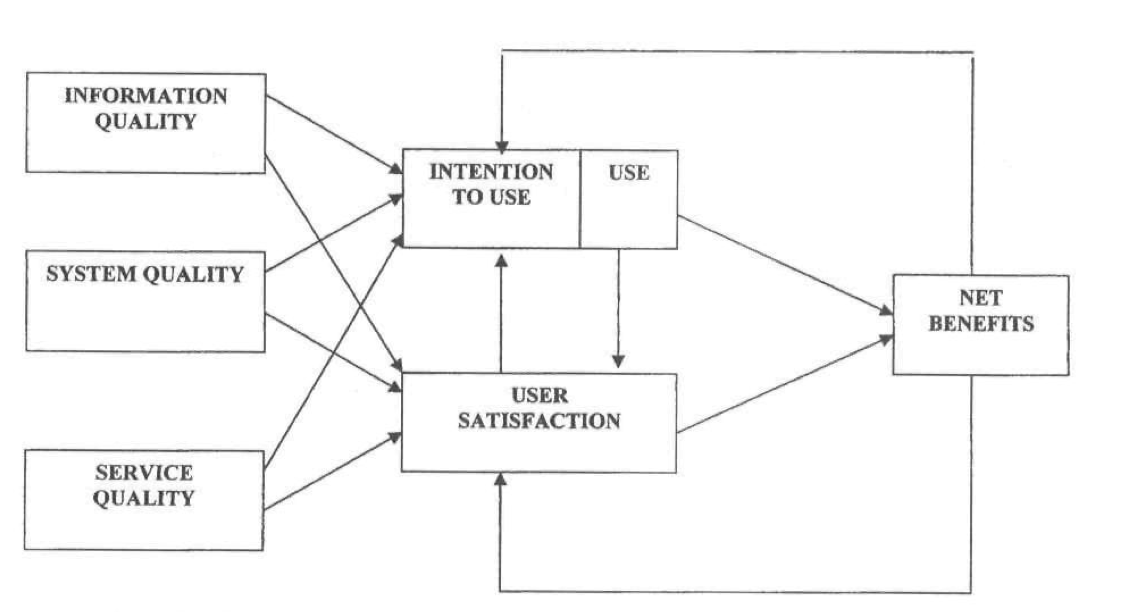
\includegraphics[width=\columnwidth, clip=true]{fig/DM-model.png}
  \caption{\emph{The Updated D \& M Success Model}}
  \label{fig:DM-model}
\end{figure}

Finally, we choose technical and social aspects to focus on, because we really want to see how it works in the usability and security for the benefits of public service, and how to improve that on the basis of the knowledge we know, which, in another word, can be seen as a investigation on the information quality, systems quality and the user satisfaction's interactive and associated ways of the Quickomat machine. In the next chapter, we will introduce two methodologies we will use in our evaluation and explain how they implement for the Quickomat evaluation. 

And as for the evaluation, it's also necessary to get a knowledge of the stakeholders. Here we are going to use the CATWOE frames firstly for this point. In IS (Information Systems), stakeholders of the system approach the same issue or process differently based on their own perspective. A common problem with it is that, if you don’t try to be precise in naming the system, you become confused as to whom is performing the activities of the system and what those activities should be. CATWOE framework is often used to produce a Root Definition for each transformation, which names the system in a structured way and making it clear who performs what task, for what purpose.

\begin{description}
  \item[Customers]
    Those who are affected by Transformation, the victim or beneficiary.
  \item[Actors]
    Those who will perform the activities involved in the transformation process.
  \item[Transformation]
    Describe the single process that will convert the input into the output.
  \item[Weltanschauung]
    The view which makes the transformation worthwhile.
  \item[Owners]
    Those who has the authority to make changes happen.
  \item[Environment]
    The constraints/restrictions which may prevent the system from operating.
\end{description}

\subsection{Technical Evaluation}
Usability describe the extent that user is enabled to perform specified goals effectively and efficiently (Melody Y. Ivory, 2001), and it is recognized as an important factor in software quality. To evaluate the usability of the information system became necessary in software system. People generally associate usability with some common attributes: learnability, efficiency, memorability, error handling, and user satisfaction (Ben Shneiderman, 1992). 

The common approach to evaluate usability is user-based test, which is conduct by a group of people and let them to work on real tasks with the system. Then how easy it is for people to perform each task are collect (Joseph S. Dumas, 1993).

Two other main categories of usability evaluation are often used in organizations. Expert-based evaluation is based on analysis of experts. With standards set beforehand, they will check if the system conform to it. An example of these methods is the famous “\emph{Heuristic Evaluation}” (Nielsen, 1994), which define a lot of guidelines as “\emph{Heuristics}”, and let evaluators examine the system according the the heuristics to check the degree that the system compliance to the guideline. Theory-based are most based on models and theories which have more formal procedures to perform the evaluation, which can get more detailed analysis of usability evaluation. One of these methods present by Z Zhang (1996) is the Goal/Question/Metric (GQM) method. In this method, goals are decomposed into tasks. Based on the models, question are designed to cover the goals. Metric are need to check the compliance of the question to the goals. The use scenario is divided to three groups: novice using, error-free expert using and error handling.

In our case study, we choose the “\emph{Heuristic Evaluation}” as our method for the reason of that it’s fast and easy to carry out, and is flexible to use. Guidelines are summarized of the design based on the research, which including dimensions, how to engage to use, privacy, the use of colors, icons and how to structure menus. By making user perform specific operation, we collect the results for analysis.

\subsubsection{Evaluation Plan}
Try to answer the question “\emph{How to test the interface-usability?}”  with choosing the approaches like “Develop a set of tasks and ask the evaluators to carry them out” or like “Provide evaluators with the goals of the system and allow them to develop their own tasks” (Nicky Danino, 2001).

\subsubsection{Choose Evaluators}
This is an important step. The more evaluators we set and choose in the process, the more usability problems we may find in the end. And also the selection of evaluators is also related with the result, which can be divided into two categories normally, those with experience and without experience (Nicky Danimo, 2001). We can also see the impact of numbers of evaluators on the proportion of usability from Figure \ref{fig:usability-problems-found}, which emphasize its important status in the heurisitic evaluation.

\begin{figure}
  \centering
  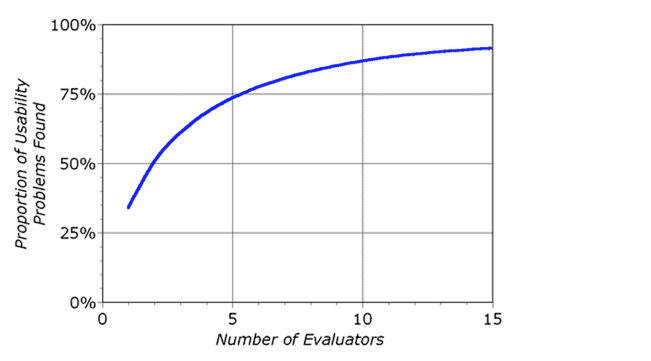
\includegraphics[width=\columnwidth, clip=true, trim=0 0 140 0]{fig/usability-problems-found.png}
  \caption{\emph{Curve showing the proportion of usability problems in an interface found by heuristic evaluation using various numbers of evaluators. (Jakob Nielson,1995)}}
  \label{fig:usability-problems-found}
\end{figure}

\subsubsection{Review Heuristics}
After above, we need to brief the evaluators about the heuristics they are going to assess. And for setting up our own heuristics, Jakob Nielson mentioned 10 general principles for interaction design (Jakob Nielson, 1995) which can be regarded as the basic rules to follow when design the heuristics.

\begin{figure}
  \centering
  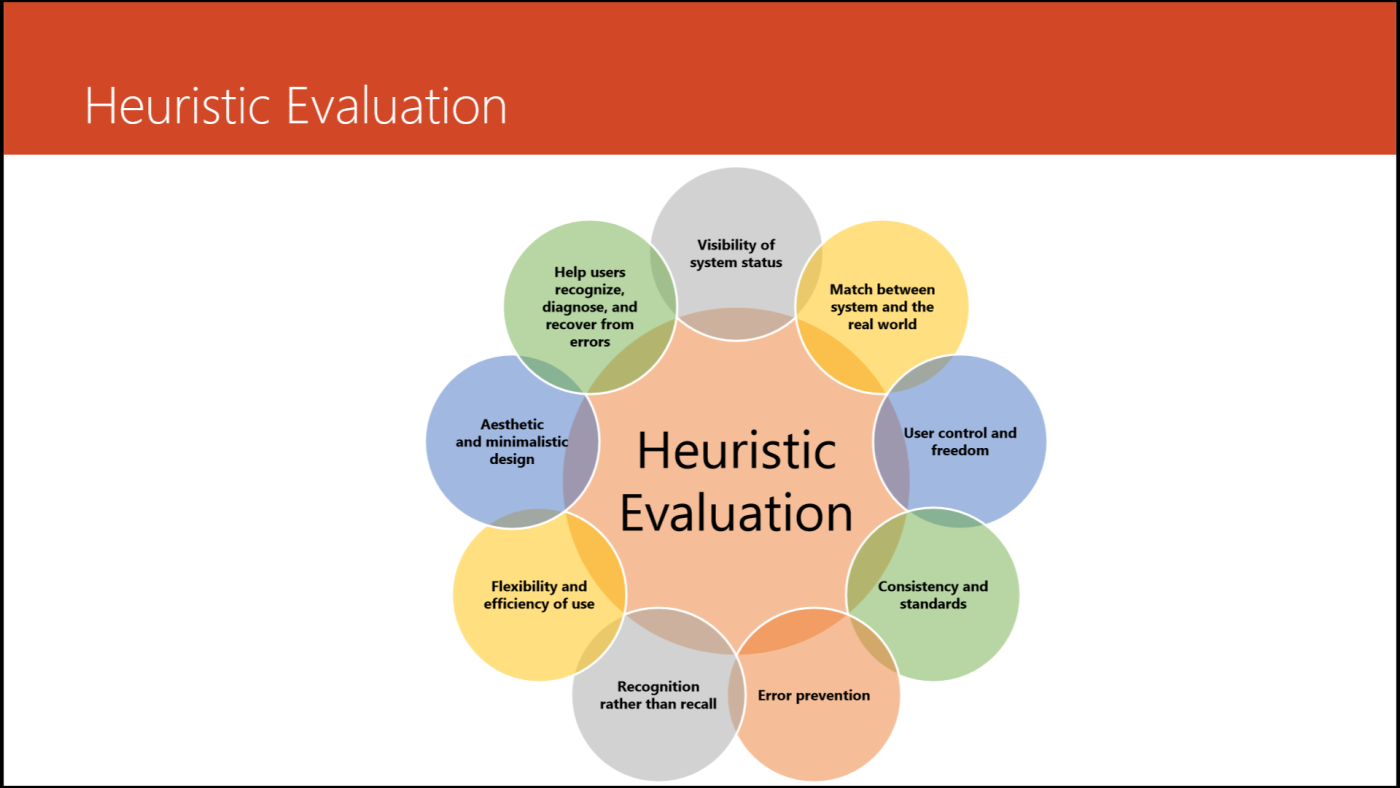
\includegraphics[width=\columnwidth, clip=true, trim=380 5 300 160]{fig/heuristic-evaluation.png}
  \caption{\emph{Jakob Nielson's 10 general principles for interaction design}}
  \label{fig:heuristic-evaluation}
\end{figure}

\begin{description}
  \item[Visibility of System Status]
    The system should always inform the users what it is undergoing.
  \item[Match between system and the real world]
    The system should provide the function of choosing national languages of users and show them in a familiar order for the users.
  \item[User control and freedom]
    Support undo, redo and quick control of the system.
  \item[Consistency and standards]
    Follow platform conventions.
  \item[Error prevention]
    Like the function that provide the users a confirmation option before they commit the action.
  \item[Recognition rather than recall]
    Minimize the users’ memory by making all the options and actions clear and visible.
  \item[Flexibility and efficiency of use]
    Allow the expert users to accelerate the process.
  \item[Aesthetic and minimalist design]
    Eliminate the irrelevant or unnecessary information in the interface or information box.
  \item[Help users recognize, diagnose, and recover from errors]
    Explain the error clearly and correctly when it occurs.
  \item[Help and documentation]
    Provide help or documentation for the better of use.
\end{description}

\subsubsection{Conduct the Evaluation}
To conduct the evaluation, the evaluators can work in groups or individually to review the interface and record the problems or findouts (Nicky Danino, 2001).

\subsubsection{Analyze the Results}
Once the evaluators have done their work, we should collect the data records from them and combine all the information with reducing the duplicated ones and address to the conclusion. And remember the golden rule “\emph{There is no such thing as a ‘user error’}” (Nicky Danino, 2001).

\subsection{Social Evaluation}
The emergence of the Quickomat not only got citizens’ attentions about its usability, but also the public influence it has brought to the society. The Quickomat now can be found at most public places such as train stations, shopping malls and universities in the south of Sweden(Quickomat AB, 2012). Taking Linköping university as an example, the university has already post it as an instruction and guide for the new students to get familiar with the life around the university (Linköpings University, 2014). 

And for the social aspect, the thing we mostly care about and want to take a deep research is about the security influence based on the emergence of the Quickomat. We try to use our own evaluation frames to find out if the Quickomat has reduce the criminal rates in the public transportation and whether the commuters, drivers and company feel safe without the cash transition. 

We use the classical data collection methods - Questionnaire and Contact Interview to help us collect the information data such as the user satisfaction about the machine now and the security extent they feel about the machine.
After that, we analyze the data and use it as a foundation for the security assessment.

\subsubsection{Methods}
%Questionnaire
Questionnaire is a classical data collection method for evaluation. A lot of questions are set for gathering the information and ideas from individuals (Evaluation briefs, 2008). Combining the security issue and questionnaire method, we design and create our own questionnaire which is suitable for the data we want to collect. And response rate is the base for the study’s analysis and conclusion. The response rate is the number of participants that responded to your questionnaire divided by the total number of participants you included in your evaluation. Obviously, higher response rates strengthen the evaluation results (Evaluation briefs, 2008). 

Based on the questionnaire and the answers from the individuals, we can take a next step for the background assessment and continue to the final security assessment.

\subsubsection{Demographic Assessment}
This section is an assessment for the basic background information of all the participants to get a full scale of the evaluation scope. The main purpose of these kinds of questions is to describe subgroups of respondents (Evaluation briefs, 2008). Limit the demographic questions to only those that are important for your analysis and cover as many as the categories of people the evaluation need.

\subsubsection{Security Assessment}
Based on the above, this section is the part that implement the evaluation of the real important issue - \emph{Security}. We prefer to assess it in an inductive way, but not in a quantitative way. By analyzing the questions and responses from the questionnaire, the assessment will start to find out what people feel or think about the public transportation security in different aspects. Also, since the assessment is undertaken both covering the quantitative number of people and many  aspects of feeling, it can be objective and reasonable.

\subsubsection{Analysis the Results}
Once we have done the assessment above, we can analyze the results we get and try to draw a conclusion of the case study.

\subsection{Economic Evaluation}
Methods that used to evaluate IT products are classified into two broad categories, first category is easily quantifiable benefits and the second is intangible benefits.

For easily quantifiable benefits, mayor methods that are used to assess IT investments include payback period and ROI. Payback period method involves calculating the number of years required for recovering the initial investment through net annual cash flow generated by the project, while ROI methods focus on computing the rate of return from an investment by considering depreciation adjusted cash inflows produced by that investment.

For intangible benefits, we often use value analysis method. Value analysis is a detailed method comprise of eight steps grouped in two phases that is focused on assessing intangible benefits of IT.

\subsection{Macro Evaluation}
Quickomat is the public welfare undertakings for urban economic development and people’s life. According to the macro evaluation, Quickomat system should be standardized by general regulations and supports. General equilibrium considerations matter more for the analysis of macro transport policy or projects with large network implications. Here, the relevant issues to consider would be broader and require at least an embryonic input-output framework to make much progress in terms of exploring the likelihood that the intervention will tend to expand or contract imperfectly competitive sectors. In addition, we develop such framework which aim to explore the nature of these aggregate relationships in more detail especially to deal with the linkages in the macro-economy and how Quickomat attracts car users to switch to public transport(Hensher, 1998).

\section{Case Study}
The following sections describe the case study that we have performed in the evaluation of  Quickomat.

\subsection{Perspectives on Evaluation}

Futhermore, from the background of the Quickomat, we managed to get the CATWOE as below.
\begin{description}
  \item[Customers]
    Traveler and others user of Quickomat are the customers. They are end user of the vending machine, and Quickomat change their way to buy tickets.
  \item[Actors]
    Quickomat AB and ÖstgötaTrafiken. They install the vending machine in public area and terminals which can process the card in places, i.e. buses.
  \item[Transformation]
    Using Quickomat can reduce the potential risk of safety compared to using cash.
  \item[Weltanschauung]
    The user now buy tickets using credit card and get tickets/card instead of cash, which will increase the safety.
  \item[Owners]
    Quickomat AB is owner, they own the system and implement it.
  \item[Environment]
    The location of the vending machine should be meet people’s need.
\end{description}

\subsection{Technical Evaluation}
The method that we described in the theoretical framework will be used in this section to check the interface-usability of the Quickomat.

\subsubsection{Evaluation Plan}
We choose to divide the evaluation into set of small tasks and ask the evaluators to carry out. Because in this way, it’s much easier to carry out and get the result we expected. And the tasks can be classified into three categories as below:
\begin{itemize}
  \item General operations on Homepage
  \item Buy / Top up the bus tickets
  \item Top up pre-paid sim card
\end{itemize}

\subsubsection{Choose Evaluators}
As for the evaluators, all of our team take part in this, since we have both kind of evaluators which are with experience and without experience in our team. Also we choose some other passengers at the Quickomat at the Hemköp in Ryds (Ryds, Linköping) to record what they do on the machine.

\subsubsection{Review Heuristics}
Based on the research and the 10 general principles for interaction design (Jakob Nielson, 1995), we study and refer some examples from the researches and draw some basic heuristics for our case.

\emph{Heuristic H1: Avoid unnecessary visual elements.} The users of the Quickomat have their own aims to perform something on the machine. So don’t make unnecessary visual elements to distract the usersfrom their purpose.

\emph{Heuristic H2: Make texts and elements visible clear.} It’s important to make the visual elements clear to the users. So user won’t take too much time to distinguish the meaning of the options. Otherwise the user may be confused and uncertain what the option means.

\emph{Heuristic H3: Support different language.} The vending machine is located in public area, and provide service not only for local people but also for tourists, international students. So the Swedish and English language need to be at least fully supported.

\emph{Heuristic H4: Show instructional videos/animation on the start page.} It’s important that the vending machine should be easily get started for novice users, so instructional videos/animation is needed to tell them how to use the machine.

\emph{Heuristic H5: Avoid unnecessary steps.} Users that use the Quickomat may be in a hurry, so try to avoid unnecessary steps. Just ask for required input from users and let them choose if they need more options instead of list all possibility every time.

\emph{Heuristic H6: Use confirm and next buttons sparingly -- provide back buttons (undo).} The machine should tolerate the mistake that the user made, and provide undo option. This can be implement either by provide previous/next option or by undo buttons.

\emph{Heuristic H7: Do not allow illegal choices.} If the textfield can only have maximum of 4 characters, don’t let user input five. When user input the illegal choices, they may receive a error in the end to remind them the mistake or just show system failure, none of which will make the right thing the user needed.

\emph{Heuristic H8: Reveal all the needed steps from the start.} This principle is to show the user where they are when they perform a specific goal. Usually this is support by the navigation bar in the bottom or top of each step, which show the current step and the number of total steps.

\subsubsection{Conduct the Evaluation}
To conduct the evaluation, the evaluators review the heuristics and record the findouts individually. The process and analysis can be seen from the next chapter with the pictures of our operations.

\subsubsection{Analysis}
\begin{description}
  \item[General operations on Homepage]
    \begin{figure}
      \centering
      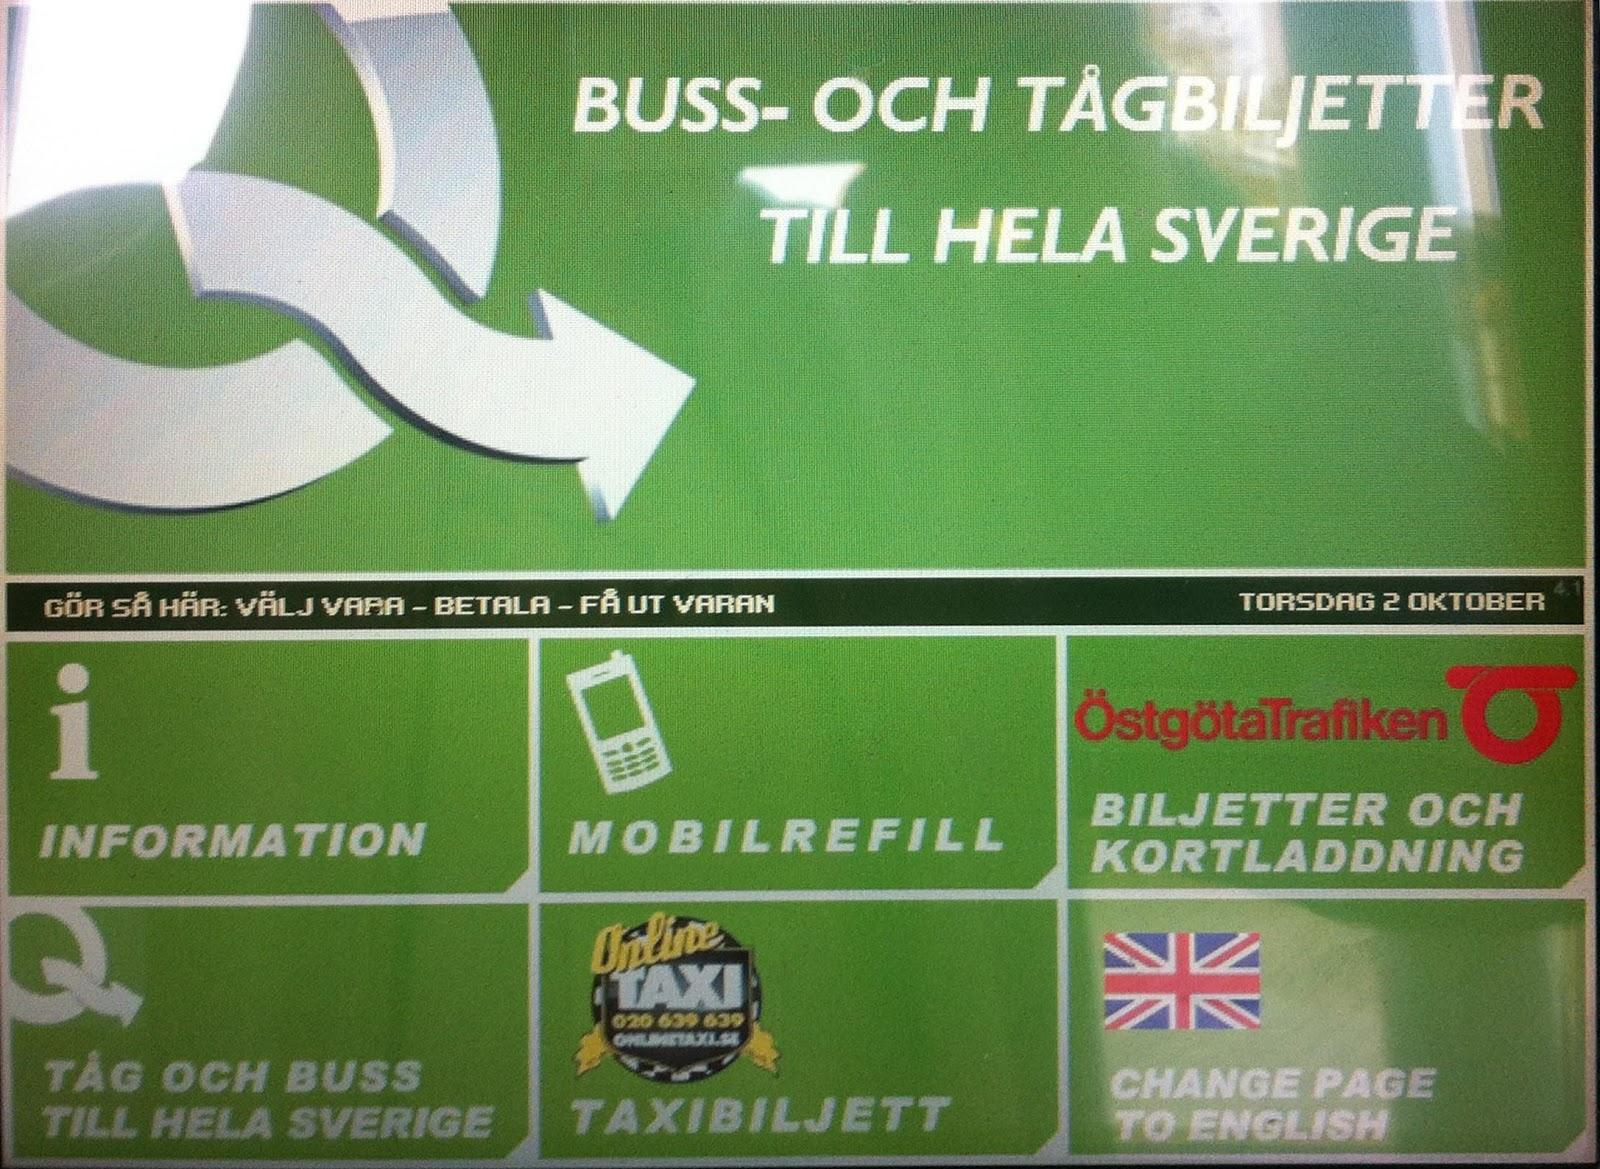
\includegraphics[width=\columnwidth]{fig/home-of-quickomat.jpg}
      \caption{Home screen of the Quickomat}
      \label{fig:home-of-quickomat}
    \end{figure}

    Figure \ref{fig:home-of-quickomat} shows the picture of the home page in Quickomat. The texts and icons are easy to distinguish, and multi-language option is support clearly at the right bottom corner of the page. The main function options occupies pretty big area so that user can easily to choose.

    However, there are no instruction video/animation for beginners. Even though that there is clear options that for people to choose, but instruction may still needed for novice user, maybe the simplest tip that indicate user can start by touch the buttons bellows is enough.

  \item[Buy/Top up bus tickets]
    \begin{figure*}
      \centering
      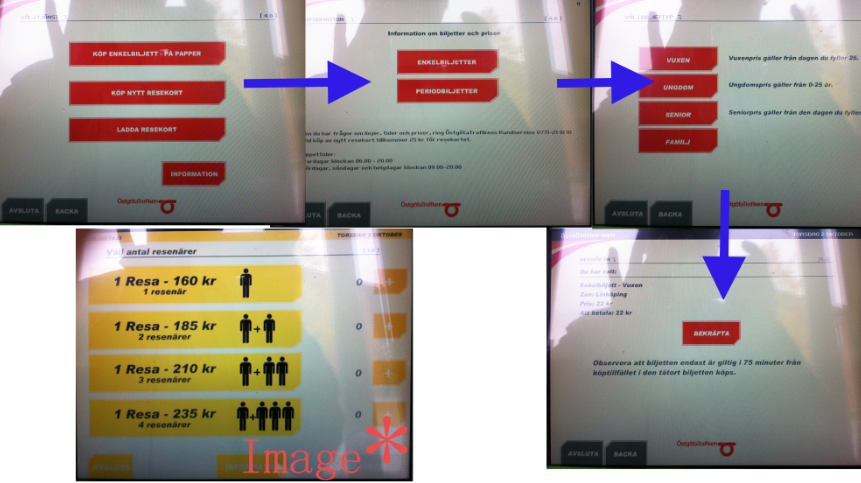
\includegraphics[width=.8\textwidth]{fig/buy-bus-ticket.png}
      \caption{The steps to buy/top up bus tickets}
      \label{fig:buy-bus-ticket}
    \end{figure*}
    Figure \ref{fig:buy-bus-ticket} shows the steps that user needed to top up or buy tickets from ÖstgötaTrafiken. The step begins by choose one type of service among buy ticket, buy card and top up card. Then comes the type of tickets including single ticket and season tickets. Detailed information of the type is show in smaller font at the bottom, which give the expert user quick choice as well as novice user enough information. Through the steps we can find that there is no step navigation in the page, which may make user confused about where they are and how many steps left in the process.

    Also we find that the type of passengers is distinguished by text. Image* shows a step that belong to another service, in which the icon of each type is well demonstrated by images of real character. So we can easily know what’s it mean. Maybe the Quickomat can improve by applying this to the similar step that user buy tickets, use different character show the types of the tickets.

  \item[Top up pre-paid sim card]
    \begin{figure*}
      \centering
      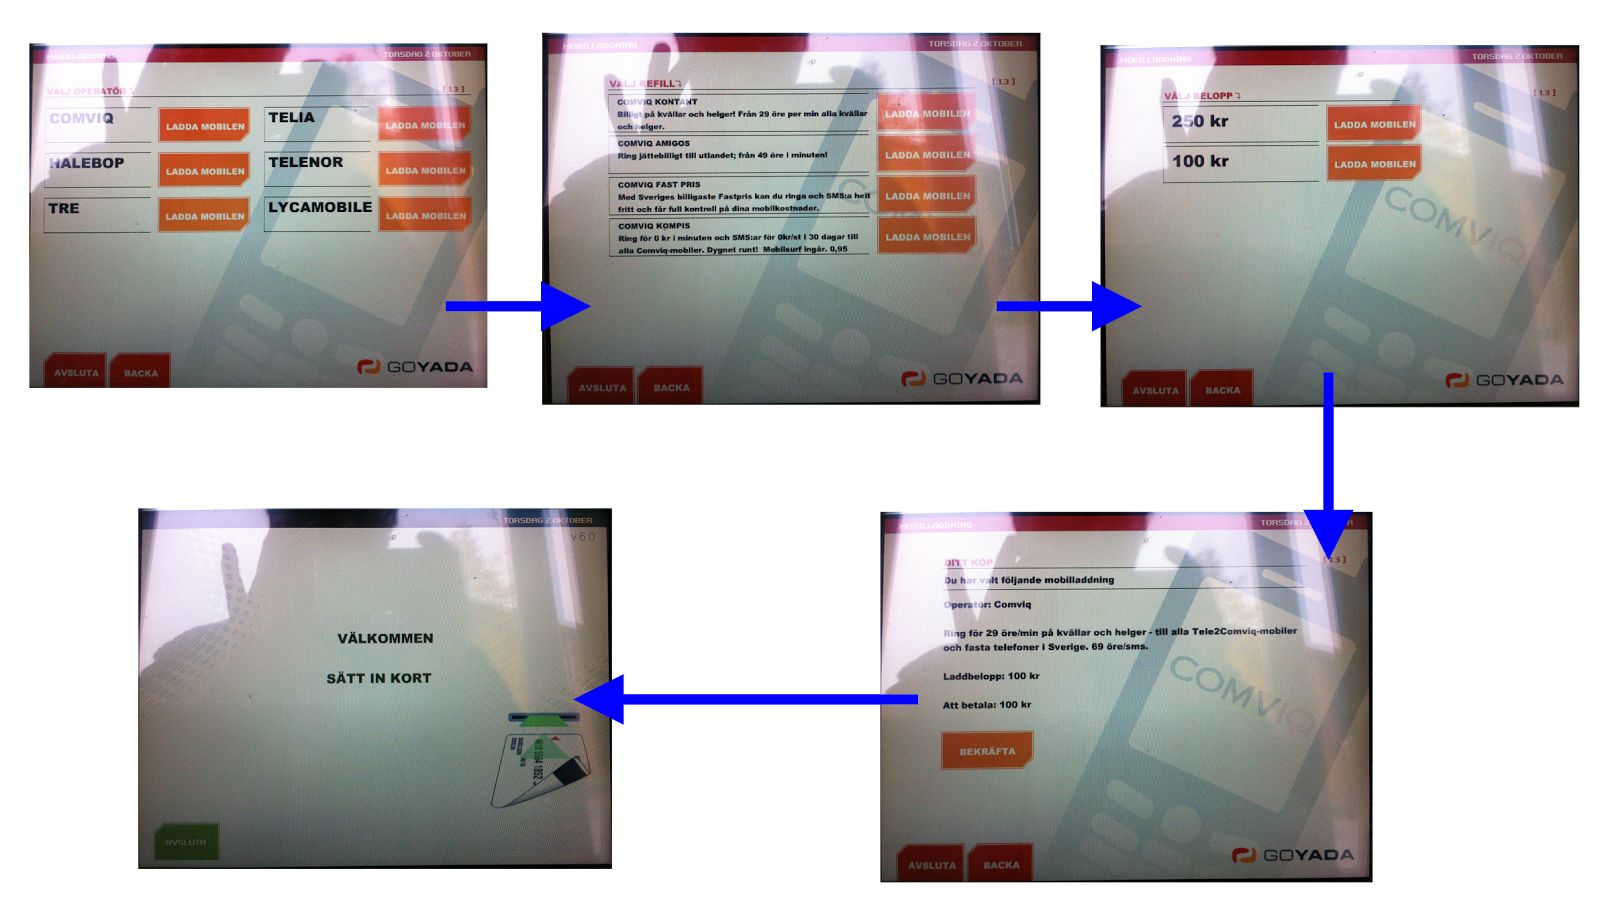
\includegraphics[width=.8\textwidth]{fig/top-up-prepaid-sim-card.png}
      \caption{The steps to top up pre-paid sim card}
      \label{fig:top-up-prepaid-sim-card}
    \end{figure*}
    Figure \ref{fig:top-up-prepaid-sim-card} shows the steps that user need to top up pre-paid sim card. The process begins by list all the operators in Sweden, when user choose one, list the detailed plans of selected operator. And then the prices of that plan, follow by a confirmation that user’s options. When user confirm the options, enter the payment process, and prompt user to insert bankcard.

    Each step has show distinguishable icons/text for user and can easily recognized. There is also undo choice for coming back to previous step to correct some options. However, there are no clear navigation that shows the progress. User don’t know where they are and how many steps they need to perform when they enter the top up process. It the improvement that Quickomat should take into consideration.
\end{description}

\subsection{Social Evaluation}

\subsubsection{Questionnaire}
The questionnaire is used in our case to collect the information about people’s opinions on the Quickomat. We hand out the questions to areas of Linkoping University, and get near 100 responses from people of different occupations, ages, genders. They have been asked about the usability and security questions about Quickomat, most questions are choices questions since they won’t take too much time to finish, and provide every possible choice for them to collect as much data as we can. The data was record into an excel file used for next section’s analyze. The questions samples are as follows:
\begin{description}
\item[Demographic Questions]
    \emph{Age, gender, occupation, the first time heard about Quickomat.}
\item[Usability Satisfaction Questions]
    \emph{What services do you often use on Quickomat?}
    \emph{What extent do you think the Quickomat has ade it easier to buy tickets?}
    \emph{...}
\item[Security Questions]
    \emph{Compared with using cash, do you think Quickomat has increased the security of public transportation?}
    \emph{Have you heard or experience any bus robbery in recent years?}
    \emph{...}
\end{description}

\subsubsection{Contact Interview}
Through our kind of email-interview with the company, we asked the questions we mostly care about and get some basic answers we want, Even though they didn't provide any solid data for us to analyze, we already felt and found out the Quickomat's great influence with the life of people living in the south of Sweden (Mvh Eva, Quickomat AB, 2014).
Like what we got from the company - Quickomat AB, they told us that the first idea of producing Quickomat, of course, was not for the security concerns. But appearently, after the emergence of Quickomat, the criminal events of public transportation has reduced a lot, especially on the drivers' personal safety. Also cancelling the cash transition between the users and the bus or train, Quickomat is providing a whole new way use of public transportation and a more safe way.

\subsubsection{Demographic Assessment}
After the stage of data collection, we carried out a plan of demographic assessment on the Quickomat based on the data we got. For a better analysis and discussion, we need to make sure that the background of the users took part in this evaluation cover all the ages,occupations or genders we planned and make it subjective and sufficient for the demostration of the result. From Figure\ref{fig:demographic-assessment} you can see the demographic distributed situation we investigate and interview on this issue, and to be specific, most of the people we got touch into are between 18 and 30 years old, which shows the phenomenon that Quickomat is popular around the people of a range of ages.
\begin{figure}
  \centering
  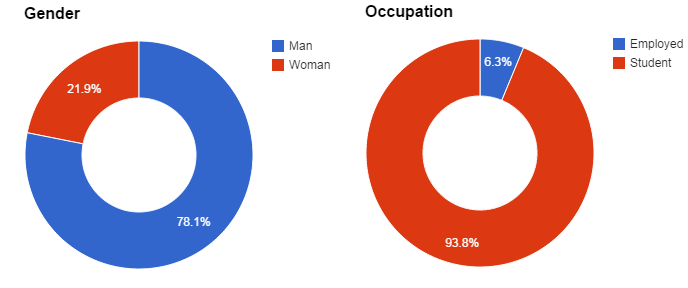
\includegraphics[width=\columnwidth]{fig/demographic-assessment.png}
  \caption{\emph{Gender,Occupation Distributed Situation}}
  \label{fig:demographic-assessment}
\end{figure}

Also, from Figure\ref{fig:demographic-assessment2}, we found out that Quickomat is a kind of product in development and improvement these years (in some public or living areas of Sweden, there is still no Quickomat yet), a lot of people have heard and used it just since the recent years. And from which, combining the interview with the Quickomat AB company, we can draw a period conlusion that the increasing numbers of users can be a sign that the users' satisfication about this IS machine has influenced by the use of it. 

\begin{figure}
  \centering
  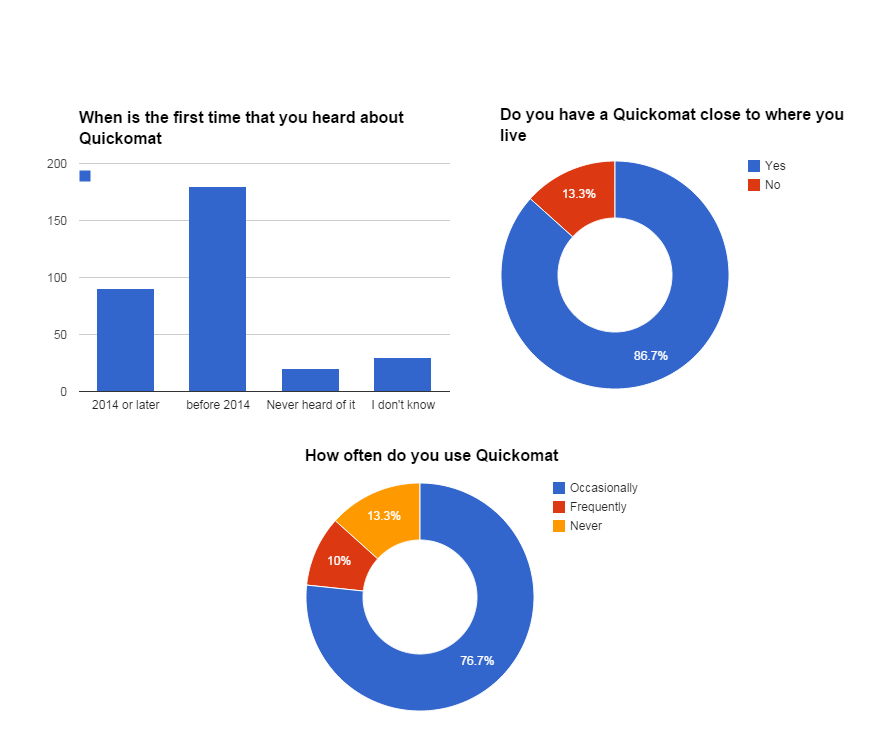
\includegraphics[width=\columnwidth]{fig/demographic-assessment2.png}
  \caption{\emph{Basic Use Distributed Situation}}
  \label{fig:demographic-assessment2}
\end{figure}

\subsubsection{Security Assessment}
Based on the above, we can get a full knowledge of the users's backgrounds, which can be the most solid foundation and support for the further security assessment. Figure \ref{fig:security-extent} shows us that the number of the people who are preferring the Quickomat as the more safety way to consume than using cash is the largest part, no matter for public transportation or pop-up their phones. And taking combination with the backgournd information together, we can be pretty much sure that the emergence of the Quickomat has changed the way that the users thinking about using cash.

\begin{figure}
  \centering
  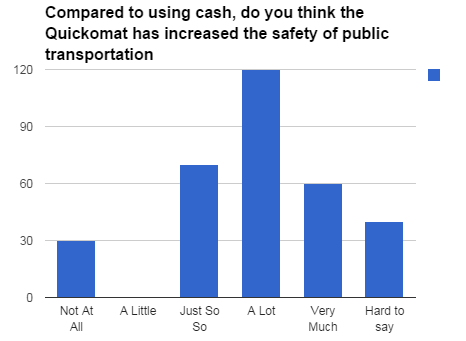
\includegraphics[width=\columnwidth]{fig/security-extent.png}
  \caption{\emph{Security-extent}}
  \label{fig:security-extent}
\end{figure}



\section{Analysis \& Discussion}
In this section we analyze and discuss the results of the case study which is closely related with the theoretical framework.

\subsection{Perspectives of Evaluation}
Based on the Updated D\&M Success Model, we can see that if we want to assess Quickomat, the interpretion of the multidimensional aspects of “use” is important and get a total understanding about the different between the atitude - “intention to use” and the behavior - “use”. For Quickomat and our research objective, “intention to use” is similiar to the expected interface-usability and feelings of security that the users want to achieve from the “use” of Quickomat. Also the “user satisfication” which is like a compliment of interface of Quickomat or the psychological confidence of feeling safe will come from the intention of using and using Quickomat. If this goes right, in contrary, both of these will increase the “user satisfication” in a way around, too.  

\subsection{Technical Evaluation}

\subsubsection{Analysis \& Discussion}
As seen the findings presented in the case study in section 3.2, we can get the difference of opinions that people hold on the interface-usability of Quickomat. Compared with other functions, most people used Quickomat buy bus tickets. And they don’t use it too often, just go to top up when needed. Most people think that Quickomat has make them easier to buy tickets or top up their phones compare to old ways. Also presented in the case , there are people who is satisfied with the functions that Quickomat provide, but don’t agree the vending machine made it easier to buy tickets since we need to go to the machine every time to top up bus card, otherwise they will be denied to take a bus since the bus don’t support cash anymore. The major of the people who are considered as none novice user and heard Quickomat for more than 1 year the system is easy to use. However, some of the people who heard Quikcomat less than 1 year report low satisfaction on the user interface of the system.

The case study that we conduct using heuristic method (Nielsen,1994) shows that most of the design is compliance with the guidelines. The system support multiple language for different people to use, use clear and big icon/text which is very easy to distinguish, provide undo function which enable the user back to previous step. However, there are also improvements that Quikcomat should make. From the questionnaire we found that people don’t have much experience, i.e novice users, are not well satisfied with the user interface of the Quickomat. Also the case study of heuristic show that instruction video/animation is needed to provide tips for novice user. Other improvements such as the progress of process in each step should be shown to user are also worth for Quickomat to take consideration.

It’s important that the usability of system should be well design to meet the user’s requirement. Our case study try to evaluation the usability and explain the improvement of the Quickomat. There are limitations that beyond our scope can be a future research direction.

\subsection{Social Evaluation}

\subsubsection{Analysis \& Discussion}
As shown in social evaluation of the case study in section 3.3, we can see the findings of different opinions and feelings assessment on the security issue that the Quickomat has brought us. Learnd from and compared with the famouse study that about “Prevalence of perceived stress, symptoms of depression and sleep disturbances in relation to information and communication technology (ICT)” (Sara Thome ́e *, Mats Eklo ̈f, Ewa Gustafsson, Ralph Nilsson, Mats Hagberg, 2005), we created our own relationship table between the Quickomat and the perceived psychological security among users, as Table below, to analyze the deep connection in this.
From which it clearly presents the perceived security or just the safety feelings among the most users. And from some perspectives, we can see that women feel more safe by using Quickomat to purchase the tickets or taking public transportation and more students than employees feel safe in this way, which proberbly means that the people without jobs are more caring about the personal security of property than the ones with payment by the companies. What's the most important is that, most of the users have started feeling it's a better and secure way to use Quickomat instead of cash transition, even though it's not the Quickomat AB's first intention of doing this (Mvh Eva, Quickomat AB, 2014).
Also as the condition that limitations in Section 1 mentioned, the research can be also reached into the area of drivers' security aspects or some other important aspects in the future.


\section{Conclusions}
From our case study, we took a relatively deep investigation and research into the Quickomat. With the help of the frameworks and classical methods, we structured the whole case study into a whole new evaluation project, and also found out some new aspects that nobody has ever done before, such as the public transportation security issue of the Quickomat. To evaluate such a vending machine, one needs to identify the specific aspects and quite a lot of qualitative and quantitative frameworks and methodologies to study and implement. 
Looking back on what we have done now, we quite refer the \emph{CATWOE} methods and \emph{Updated DM Success Model} in the beginning to analyze the basic points and backgournd information we need to understand and achieve in this evaluation, like the stakeholders and the relationships between the quality of systems, service and information and use, user satisfaction, which helps us identify the benefits of the Quickomat and found a solid base for further study. 
In the process, we chose technical and social perspectives as our main aspects for the evaluation, which speparately conducted by the methods of classical \emph{Heuristic Methods} and \emph{Questionnaire-Interview-Based Methods}. During the period of case study, we evaluate the Quickomat just from the aspects we had set up and implemented the methods very well in the case. That's really helpul for the data collection and analysis for the further study. Our analysis can be concluded that the interface-usability of the Quickomat has reached an acceptable level for the normal users. And also for the security part it's quite a safety way to use Quickomat nowadays in some areas of Sweden and we hope to keep looking up into this area in the next period of study since it's a very interesting and meaningful aspect.
Therefore, we suggested that the future research focus on the security issue of drivers or some other detaile criminal rates related with the Quickomat, since we kind of have a short time frame and can't get any detailed information from public sectors this time. It should be a good idea to look deeper in this part as it's a part of concern of the regular life of the people in Sweden.


\section{Summary}

% Bibliography
\cite{*}
\bibliographystyle{plainnat}
\bibliography{tddc34-report-stockholm-quickomat}
\end{document}